\subsection{Deskryptory wykresu \PP{}}


Następna techniką z domeny czasowej wykorzystywaną do analizy HRV to technika opierająca
się na tzw. wykresach \PP{}.

Wykres \PP{}, którego nazwa pochodzi od twórcy tej techniki Henri \PP{}, jest\\ 
analityczno-wizualną technika ułatwiającą analizę złożonych zjawisk i ma ona zastosowanie
nie tylko w naukach medycznych ale także m.in. w meteorologii, geofizyce, astronomii \cite{ott}.
Element wizualny wynika z użycia odpowiednio przygotowanych wykresów i w praktyce jest to
bardzo ważny element gdyż umożliwia na bardzo szybką wstępna jakościową analizę danego
zjawiska. Element analityczny jest związany z parametrami, tak zwanymi deskryptorami,
które wyrażają ilościowo informacje zawarte w wykresie \PP{}. Należy zaznaczyć że
metod ta jest bardzo odporna na dane zawierające artefakty lub wartości odstające i w
tym sensie ma przewagę nad technikami które wymagają niezakłóconych danych np 
wykorzystujące szybką transformatę Fouriera (FFT).

Konstrukcja wykresów \PP{} jest dość prosta, przyjmując że szereg $RR$ wyrazimy jako
wektor:
\begin{equation}
\bRR = (RR_{1}, RR_{2}, \ldots, RR_{n})
\end{equation}
oś odciętych jest utworzona z wektora $RR$ bez ostatniego elementu, natomiast oś rzędnych
zawiera elementy bezpośrednio po nich następujące, czyli wektor $RR$ bez elementu
pierwszego:
\begin{equation}
\bRRm = (RR_{1}, RR_{2}, \ldots, RR_{n-1}),
\bRRn = (RR_{2}, RR_{2}, \ldots, RR_{n})
\label{eq:wektory2} 
\end{equation}
lub inaczej
\begin{equation}
  \mathcal{P} = \{(RR_1, RR_2),\ldots, (RR_i, RR_{i+1}), (RR_{n-1}, RR_n )\},
 \label{eq:p_plot}
\end{equation}
zatem wykres \PP{} jest zbiorem (chmurą) punktów $(RR_{i}, RR_{i+1})$ gdzie $i=(1, \ldots, n-1)$

Podstawowymi parametrami (deskryptorami) utworzonymi w oparciu o powyższą reprezentacją 
graficzną wektora $\bRR$ są parametry określane w literaturze symbolami $SD1$ i $SD2$, które
wyrażają odpowiednio zmienność krótko- i długoterminową rytmu serca.
%matematycznie wyrażonymi przy pomocy wariancji:

%\begin{equation}
%SD1^2 = Var\left(\frac{\bRRn - \bRRm}{\sqrt{2}}\right)
%\end{equation}

%\begin{equation}
%SD2^2 = Var\left(\frac{\bRRn + \bRRm}{\sqrt{2}}\right)
%\end{equation}

%Tak zdefiniowane~jak powyżej
Parametry $SD1$, $SD2$ mierzą rozproszenie punktów wykresu
\PP{} względem odpowiednio tzw linii identyczności $l_{I}$ (linii dla której $\bRRm = \bRRn$)
oraz linii prostopadłej do linii identyczności $l_2$ przechodzącej przez centroid. Na
rysunku \ref{fig:pp_distrib} została przedstawiona konstrukcja tych parametrów oraz zostały
przedstawione rzuty wariancji: histogram (a) krótkoterminowej zmienności rytmu serca $SD1$
wzdłuż linii identyczności $l_{I}$, histogram (b) pełnej zmienności rytmu serca na oś $RR_n$,
histogram (c) długoterminowej zmienności rytmu serca $SD2$ wzdłuż linii prostopadłej $l_2$
do linii identyczności $l_{I}$.

Jeśli zdefiniujemy szeregi różnic i sum współrzędnych punktów obróconego PP za pomocą
relacji:


\begin{equation}
\mathbf{L_1} = \left \{ \frac{RR_1 - RR_{2}}{\sqrt{2}}, \ldots, \frac{RR_i - RR_{i+1}}{\sqrt{2}}, \ldots, \frac{RR_{n-1} - RR_{n}}{\sqrt{2}} \right \},
\end{equation}
\begin{equation}
\mathbf{L_2} = \left \{\frac{RR_1 + RR_{2}}{\sqrt{2}}, \ldots, \frac{RR_i + RR_{i+1}}{\sqrt{2}}, \ldots, \frac{RR_{n-1} + RR_{n}}{\sqrt{2}} \right \},
\end{equation}
a~sam obrót jako:
\begin{equation}
\left[
    \begin{array}{c}
      x_i\\
      y_i\\
    \end{array} \right] 
  = 
\left[ \begin{array}{c c}
      \cos(\frac{\pi}{4}) & -\sin(\frac{\pi}{4})\\
      \sin(\frac{\pi}{4}) & \cos(\frac{\pi}{4})\\
    \end{array} \right] 
\left[
    \begin{array}{c}
      \mbox{RR}_i\\
      \mbox{RR}_{i+1}\\
    \end{array} \right],
\end{equation}
to parametry $SD1$ i $SD2$ możemy wyrazić jako wariancje szeregów $\mathbf{L_1}$ i $\mathbf{L_2}$ \cite{poinc_jaro,jarek2}:
\begin{equation}
  SD1^2 = \mbox{Var}( \mathbf{L_1})
  = \mbox{Var}\left(\frac{\bRRn - \bRRp}{\sqrt{2}}\right),
  \label{eq:sd1}
\end{equation}
\begin{equation}
  SD2^2 = \mbox{Var}( \mathbf{L_2})
  = \mbox{Var}\left(\frac{\bRRn + \bRRp}{\sqrt{2}}\right). 
  \label{eq:sd2}
\end{equation}

\begin{figure}
\centering
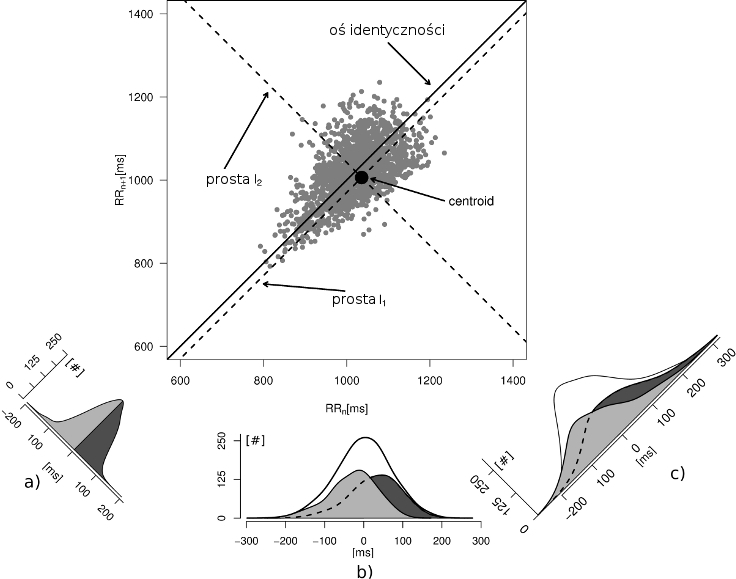
\includegraphics[width=\textwidth]{graph/pp_distrib.jpg}
\caption{Rysunek prezentuje położenie prostej równoległej ($l_1$) i~prostej prostopodłej ($l_2$) do osi identyczności separującej punkty reprezentujące skrócenia i~wydłużenia odstępów $RR$. Na wykresie przedstawiono również rozkłady punktów opisujących zmienność krótkoterminową $SD1$ (panel $a$ - rzut PP na oś $l_2$), zmienność długoterminową $SD2$ (panel $c$ reprezentujący rzut PP na oś $l_1$) oraz zmieność całkowitą (panel $b$ -- rzut PP na oś odciętych). Na histogramach różnymi odcieniami szarości oznaczono wkłady pochodzące od punktów, znajdujących się nad i~pod osią identyczności. Opracowano na podstawie \cite{hrstruct} -- rysunek udostępniony przez Jarosława Piskorskiego i~Przemysława Guzika na licencji CC BY.}
\label{fig:pp_distrib}
\end{figure}

Poniżej jeszcze inna postać na wariancje $SD1$ i $SD2$ tym razem oparta na własnościach geometrycznych linii identyczności występującej na rysunku \ref{fig:pp_distrib}: 

\begin{equation}
SD1^2 = \frac{1}{n}\sum_{i=1}^{n}r_{i}^{\perp 2}
\end{equation}

\begin{equation}
SD2^2 = \frac{1}{n}\sum_{i=1}^{n}r_{i}^{\parallel 2}
\end{equation}

gdzie $r_{i}^{\perp}$ jest prostopadłą odległością punktu $(RR_{i}, RR_{i+1})$ do linii
identyczności, $r_{i}^{\parallel}$ jest odległością punktu $(RR_{i}, RR_{i+1})$ do linii
$l_2$ wzdłuż linii identyczności.

Należy zaznaczyć że wyrażenie (\ref{eq:sd1}) dla krótkoterminowej zmienności rytmu serca
nie jest z matematycznego punktu widzenia odchyleniem standardowym, gdyż nie jest
wyznaczane względem linii $l_1$ przechodzącej przez centroid, to znaczy nie minimalizuje
drugiego momentu rozkładu punktów $RR$. Jednakże to w żaden sposób
nie umniejsza użyteczności tego deskryptora i to z dwóch powodów: (1) linia
identyczności dzieli cały wykres \PP{} na dwie części, górną dotyczącą zwolnień,
dolną dotyczącą przyspieszeń, zatem $SD1$ liczona względem $l_{I}$ ma wyraźną interpretację
fizjologiczną, (2) różnica pomiędzy wariancjami odnoszącymi się odpowiednio do linii $l_1$
oraz $l_{I}$ zgodnie z wartościami podanymi w \cite{poinc_jaro} jest rzędu $10^{-5}$ i
dąży do $0$ dla coraz większej liczby pomiarów, ponadto sam błąd związany z wprowadzeniem
wariancji względem $l_{I}$ jest rzędu $10^{-8}$, zatem w praktyce jest zaniedbywalny.

Relacja pomiędzy krótkoterminową i długoterminową zmiennością rytmu serca opisanymi powyżej
a miarą pełnej zmienności rytmu serca opisanej w \ref{subsec:pelna_zmiennosc}
jest następująca:
\begin{equation}
SDNN^2 = \frac{1}{2}(SD1^2 + SD2^2)\label{SDNNpartitioning}.
\end{equation}